% Options for packages loaded elsewhere
\PassOptionsToPackage{unicode}{hyperref}
\PassOptionsToPackage{hyphens}{url}
%
\documentclass[
]{article}
\usepackage{lmodern}
\usepackage{amssymb,amsmath}
\usepackage{ifxetex,ifluatex}
\ifnum 0\ifxetex 1\fi\ifluatex 1\fi=0 % if pdftex
  \usepackage[T1]{fontenc}
  \usepackage[utf8]{inputenc}
  \usepackage{textcomp} % provide euro and other symbols
\else % if luatex or xetex
  \usepackage{unicode-math}
  \defaultfontfeatures{Scale=MatchLowercase}
  \defaultfontfeatures[\rmfamily]{Ligatures=TeX,Scale=1}
\fi
% Use upquote if available, for straight quotes in verbatim environments
\IfFileExists{upquote.sty}{\usepackage{upquote}}{}
\IfFileExists{microtype.sty}{% use microtype if available
  \usepackage[]{microtype}
  \UseMicrotypeSet[protrusion]{basicmath} % disable protrusion for tt fonts
}{}
\makeatletter
\@ifundefined{KOMAClassName}{% if non-KOMA class
  \IfFileExists{parskip.sty}{%
    \usepackage{parskip}
  }{% else
    \setlength{\parindent}{0pt}
    \setlength{\parskip}{6pt plus 2pt minus 1pt}}
}{% if KOMA class
  \KOMAoptions{parskip=half}}
\makeatother
\usepackage{xcolor}
\IfFileExists{xurl.sty}{\usepackage{xurl}}{} % add URL line breaks if available
\IfFileExists{bookmark.sty}{\usepackage{bookmark}}{\usepackage{hyperref}}
\hypersetup{
  pdftitle={TP 2},
  pdfauthor={Nantas Paul - Poupard Paul - Spriet Thibault - Ung Théophile},
  hidelinks,
  pdfcreator={LaTeX via pandoc}}
\urlstyle{same} % disable monospaced font for URLs
\usepackage[margin=1in]{geometry}
\usepackage{color}
\usepackage{fancyvrb}
\newcommand{\VerbBar}{|}
\newcommand{\VERB}{\Verb[commandchars=\\\{\}]}
\DefineVerbatimEnvironment{Highlighting}{Verbatim}{commandchars=\\\{\}}
% Add ',fontsize=\small' for more characters per line
\usepackage{framed}
\definecolor{shadecolor}{RGB}{248,248,248}
\newenvironment{Shaded}{\begin{snugshade}}{\end{snugshade}}
\newcommand{\AlertTok}[1]{\textcolor[rgb]{0.94,0.16,0.16}{#1}}
\newcommand{\AnnotationTok}[1]{\textcolor[rgb]{0.56,0.35,0.01}{\textbf{\textit{#1}}}}
\newcommand{\AttributeTok}[1]{\textcolor[rgb]{0.77,0.63,0.00}{#1}}
\newcommand{\BaseNTok}[1]{\textcolor[rgb]{0.00,0.00,0.81}{#1}}
\newcommand{\BuiltInTok}[1]{#1}
\newcommand{\CharTok}[1]{\textcolor[rgb]{0.31,0.60,0.02}{#1}}
\newcommand{\CommentTok}[1]{\textcolor[rgb]{0.56,0.35,0.01}{\textit{#1}}}
\newcommand{\CommentVarTok}[1]{\textcolor[rgb]{0.56,0.35,0.01}{\textbf{\textit{#1}}}}
\newcommand{\ConstantTok}[1]{\textcolor[rgb]{0.00,0.00,0.00}{#1}}
\newcommand{\ControlFlowTok}[1]{\textcolor[rgb]{0.13,0.29,0.53}{\textbf{#1}}}
\newcommand{\DataTypeTok}[1]{\textcolor[rgb]{0.13,0.29,0.53}{#1}}
\newcommand{\DecValTok}[1]{\textcolor[rgb]{0.00,0.00,0.81}{#1}}
\newcommand{\DocumentationTok}[1]{\textcolor[rgb]{0.56,0.35,0.01}{\textbf{\textit{#1}}}}
\newcommand{\ErrorTok}[1]{\textcolor[rgb]{0.64,0.00,0.00}{\textbf{#1}}}
\newcommand{\ExtensionTok}[1]{#1}
\newcommand{\FloatTok}[1]{\textcolor[rgb]{0.00,0.00,0.81}{#1}}
\newcommand{\FunctionTok}[1]{\textcolor[rgb]{0.00,0.00,0.00}{#1}}
\newcommand{\ImportTok}[1]{#1}
\newcommand{\InformationTok}[1]{\textcolor[rgb]{0.56,0.35,0.01}{\textbf{\textit{#1}}}}
\newcommand{\KeywordTok}[1]{\textcolor[rgb]{0.13,0.29,0.53}{\textbf{#1}}}
\newcommand{\NormalTok}[1]{#1}
\newcommand{\OperatorTok}[1]{\textcolor[rgb]{0.81,0.36,0.00}{\textbf{#1}}}
\newcommand{\OtherTok}[1]{\textcolor[rgb]{0.56,0.35,0.01}{#1}}
\newcommand{\PreprocessorTok}[1]{\textcolor[rgb]{0.56,0.35,0.01}{\textit{#1}}}
\newcommand{\RegionMarkerTok}[1]{#1}
\newcommand{\SpecialCharTok}[1]{\textcolor[rgb]{0.00,0.00,0.00}{#1}}
\newcommand{\SpecialStringTok}[1]{\textcolor[rgb]{0.31,0.60,0.02}{#1}}
\newcommand{\StringTok}[1]{\textcolor[rgb]{0.31,0.60,0.02}{#1}}
\newcommand{\VariableTok}[1]{\textcolor[rgb]{0.00,0.00,0.00}{#1}}
\newcommand{\VerbatimStringTok}[1]{\textcolor[rgb]{0.31,0.60,0.02}{#1}}
\newcommand{\WarningTok}[1]{\textcolor[rgb]{0.56,0.35,0.01}{\textbf{\textit{#1}}}}
\usepackage{graphicx,grffile}
\makeatletter
\def\maxwidth{\ifdim\Gin@nat@width>\linewidth\linewidth\else\Gin@nat@width\fi}
\def\maxheight{\ifdim\Gin@nat@height>\textheight\textheight\else\Gin@nat@height\fi}
\makeatother
% Scale images if necessary, so that they will not overflow the page
% margins by default, and it is still possible to overwrite the defaults
% using explicit options in \includegraphics[width, height, ...]{}
\setkeys{Gin}{width=\maxwidth,height=\maxheight,keepaspectratio}
% Set default figure placement to htbp
\makeatletter
\def\fps@figure{htbp}
\makeatother
\setlength{\emergencystretch}{3em} % prevent overfull lines
\providecommand{\tightlist}{%
  \setlength{\itemsep}{0pt}\setlength{\parskip}{0pt}}
\setcounter{secnumdepth}{-\maxdimen} % remove section numbering
\usepackage[utf8]{inputenc}
\usepackage{booktabs}
\usepackage{longtable}
\usepackage{array}
\usepackage{multirow}
\usepackage{wrapfig}
\usepackage{float}
\usepackage{colortbl}
\usepackage{pdflscape}
\usepackage{tabu}
\usepackage{threeparttable}
\usepackage{threeparttablex}
\usepackage[normalem]{ulem}
\usepackage{makecell}
\usepackage{xcolor}

\title{TP 2}
\usepackage{etoolbox}
\makeatletter
\providecommand{\subtitle}[1]{% add subtitle to \maketitle
  \apptocmd{\@title}{\par {\large #1 \par}}{}{}
}
\makeatother
\subtitle{TP-2: Droite de Marchés des Capitaux}
\author{Nantas Paul - Poupard Paul - Spriet Thibault - Ung Théophile}
\date{Février 2021}

\begin{document}
\maketitle

\hypertarget{donnuxe9es}{%
\section{Données}\label{donnuxe9es}}

\hypertarget{suxe9ries-de-rendement-quatidien-pour-11-valeurs}{%
\subsection{Séries de rendement quatidien pour 11
valeurs:}\label{suxe9ries-de-rendement-quatidien-pour-11-valeurs}}

\begin{Shaded}
\begin{Highlighting}[]
\NormalTok{daily.ret.file <-}\StringTok{ }\KeywordTok{file.path}\NormalTok{(}\KeywordTok{get.data.folder}\NormalTok{(), }\StringTok{"daily.ret.rda"}\NormalTok{)}
\KeywordTok{load}\NormalTok{(daily.ret.file)}
\KeywordTok{kable}\NormalTok{(}\KeywordTok{table.Stats}\NormalTok{(daily.ret), }\StringTok{"latex"}\NormalTok{, }\DataTypeTok{booktabs=}\NormalTok{T) }\OperatorTok\StringTok{ }\KeywordTok{kable_styling}\NormalTok{(}\DataTypeTok{latex_options=}\StringTok{"scale_down"}\NormalTok{)}
\end{Highlighting}
\end{Shaded}

\begin{table}[H]
\centering
\resizebox{\linewidth}{!}{
\begin{tabular}{lrrrrrrrrrrr}
\toprule
  & AAPL & AMZN & MSFT & F & SPY & QQQ & XOM & MMM & HD & PG & KO\\
\midrule
Observations & 3308.0000 & 3308.0000 & 3308.0000 & 3308.0000 & 3308.0000 & 3308.0000 & 3308.0000 & 3308.0000 & 3308.0000 & 3308.0000 & 3308.0000\\
NAs & 0.0000 & 0.0000 & 0.0000 & 0.0000 & 0.0000 & 0.0000 & 0.0000 & 0.0000 & 0.0000 & 0.0000 & 0.0000\\
Minimum & -0.1792 & -0.1278 & -0.1171 & -0.2500 & -0.0984 & -0.0896 & -0.1395 & -0.1295 & -0.0822 & -0.0790 & -0.0867\\
Quartile 1 & -0.0077 & -0.0094 & -0.0073 & -0.0103 & -0.0038 & -0.0047 & -0.0068 & -0.0055 & -0.0067 & -0.0046 & -0.0047\\
Median & 0.0010 & 0.0008 & 0.0005 & 0.0000 & 0.0006 & 0.0010 & 0.0001 & 0.0008 & 0.0006 & 0.0004 & 0.0007\\
\addlinespace
Arithmetic Mean & 0.0012 & 0.0015 & 0.0008 & 0.0005 & 0.0004 & 0.0006 & 0.0001 & 0.0004 & 0.0008 & 0.0004 & 0.0005\\
Geometric Mean & 0.0010 & 0.0012 & 0.0006 & 0.0001 & 0.0003 & 0.0005 & 0.0000 & 0.0003 & 0.0006 & 0.0003 & 0.0004\\
Quartile 3 & 0.0112 & 0.0123 & 0.0088 & 0.0106 & 0.0056 & 0.0070 & 0.0073 & 0.0070 & 0.0082 & 0.0055 & 0.0059\\
Maximum & 0.1390 & 0.2695 & 0.1860 & 0.2952 & 0.1452 & 0.1216 & 0.1719 & 0.0988 & 0.1407 & 0.1021 & 0.1388\\
SE Mean & 0.0003 & 0.0004 & 0.0003 & 0.0005 & 0.0002 & 0.0002 & 0.0003 & 0.0002 & 0.0003 & 0.0002 & 0.0002\\
\addlinespace
LCL Mean (0.95) & 0.0005 & 0.0006 & 0.0002 & -0.0005 & 0.0000 & 0.0002 & -0.0004 & -0.0001 & 0.0002 & 0.0000 & 0.0001\\
UCL Mean (0.95) & 0.0019 & 0.0023 & 0.0013 & 0.0014 & 0.0008 & 0.0011 & 0.0006 & 0.0009 & 0.0013 & 0.0007 & 0.0009\\
Variance & 0.0004 & 0.0006 & 0.0003 & 0.0007 & 0.0001 & 0.0002 & 0.0002 & 0.0002 & 0.0003 & 0.0001 & 0.0001\\
Stdev & 0.0196 & 0.0243 & 0.0170 & 0.0266 & 0.0121 & 0.0130 & 0.0150 & 0.0140 & 0.0162 & 0.0109 & 0.0113\\
Skewness & -0.2151 & 1.4889 & 0.4319 & 0.7627 & 0.1379 & -0.0084 & 0.4199 & -0.3815 & 0.5114 & 0.0555 & 0.5004\\
\addlinespace
Kurtosis & 6.2706 & 16.8872 & 10.2176 & 20.9458 & 15.2824 & 7.3976 & 15.4203 & 7.3856 & 6.4641 & 8.1017 & 14.3236\\
\bottomrule
\end{tabular}}
\end{table}

\hypertarget{rendement-annuel-moyen}{%
\subsection{Rendement annuel moyen:}\label{rendement-annuel-moyen}}

\begin{Shaded}
\begin{Highlighting}[]
\KeywordTok{kable}\NormalTok{(}\DecValTok{252}\OperatorTok{*}\DecValTok{100}\OperatorTok{*}\KeywordTok{colMeans}\NormalTok{(daily.ret), }\StringTok{"latex"}\NormalTok{, }\DataTypeTok{booktabs=}\NormalTok{T, }\DataTypeTok{digits=}\DecValTok{1}\NormalTok{, }\DataTypeTok{col.names=}\KeywordTok{c}\NormalTok{(}\StringTok{"Rendement (%)"}\NormalTok{), }
      \DataTypeTok{caption=}\StringTok{"Rendement annuel moyen"}\NormalTok{)}
\end{Highlighting}
\end{Shaded}

\begin{table}

\caption{\label{tab:unnamed-chunk-2}Rendement annuel moyen}
\centering
\begin{tabular}[t]{lr}
\toprule
  & Rendement (\%)\\
\midrule
AAPL & 30.2\\
AMZN & 37.2\\
MSFT & 19.0\\
F & 11.4\\
SPY & 9.9\\
\addlinespace
QQQ & 15.3\\
XOM & 3.5\\
MMM & 9.9\\
HD & 19.2\\
PG & 9.3\\
\addlinespace
KO & 12.5\\
\bottomrule
\end{tabular}
\end{table}

\hypertarget{matrice-de-corruxe9lation-des-rendements}{%
\subsection{Matrice de corrélation des
rendements:}\label{matrice-de-corruxe9lation-des-rendements}}

\begin{Shaded}
\begin{Highlighting}[]
\NormalTok{correl <-}\StringTok{ }\KeywordTok{cor}\NormalTok{(daily.ret)}
\NormalTok{correl[}\KeywordTok{lower.tri}\NormalTok{(correl)] <-}\StringTok{ }\OtherTok{NA}
\KeywordTok{options}\NormalTok{(}\DataTypeTok{knitr.kable.NA =} \StringTok{''}\NormalTok{)}
\KeywordTok{kable}\NormalTok{(correl, }\StringTok{"latex"}\NormalTok{, }\DataTypeTok{booktabs=}\NormalTok{T, }\DataTypeTok{digits=}\DecValTok{2}\NormalTok{, }\DataTypeTok{caption=}\StringTok{"Corrélation des rendements quotidiens"}\NormalTok{) }\OperatorTok
\KeywordTok{kable_styling}\NormalTok{(}\DataTypeTok{latex_options=}\StringTok{"scale_down"}\NormalTok{)}
\end{Highlighting}
\end{Shaded}

\begin{table}

\caption{\label{tab:unnamed-chunk-3}Corrélation des rendements quotidiens}
\centering
\resizebox{\linewidth}{!}{
\begin{tabular}[t]{lrrrrrrrrrrr}
\toprule
  & AAPL & AMZN & MSFT & F & SPY & QQQ & XOM & MMM & HD & PG & KO\\
\midrule
AAPL & 1 & 0.46 & 0.49 & 0.37 & 0.61 & 0.75 & 0.40 & 0.45 & 0.42 & 0.32 & 0.32\\
AMZN &  & 1.00 & 0.50 & 0.33 & 0.56 & 0.66 & 0.39 & 0.41 & 0.44 & 0.27 & 0.30\\
MSFT &  &  & 1.00 & 0.39 & 0.71 & 0.76 & 0.53 & 0.53 & 0.49 & 0.44 & 0.46\\
F &  &  &  & 1.00 & 0.56 & 0.53 & 0.37 & 0.44 & 0.46 & 0.30 & 0.31\\
SPY &  &  &  &  & 1.00 & 0.92 & 0.77 & 0.75 & 0.71 & 0.62 & 0.60\\
\addlinespace
QQQ &  &  &  &  &  & 1.00 & 0.64 & 0.69 & 0.66 & 0.52 & 0.52\\
XOM &  &  &  &  &  &  & 1.00 & 0.60 & 0.47 & 0.52 & 0.49\\
MMM &  &  &  &  &  &  &  & 1.00 & 0.55 & 0.50 & 0.47\\
HD &  &  &  &  &  &  &  &  & 1.00 & 0.45 & 0.44\\
PG &  &  &  &  &  &  &  &  &  & 1.00 & 0.57\\
\addlinespace
KO &  &  &  &  &  &  &  &  &  &  & 1.00\\
\bottomrule
\end{tabular}}
\end{table}

\hypertarget{droite-de-marchuxe9-des-capitaux-capital-market-line}{%
\section{Droite de Marché des Capitaux (Capital Market
Line)}\label{droite-de-marchuxe9-des-capitaux-capital-market-line}}

\begin{itemize}
\tightlist
\item
  A partir des calculs présentés en cours, mettre en oeuvre une méthode
  numérique pour déterminer le portefeuille tangent quand les poids des
  actifs risqués sont contraints à être positifs: \(w_i \ge 0\).
\end{itemize}

\hypertarget{portefeuille-uxe0-variance-minimale}{%
\subsection{Portefeuille à Variance
Minimale}\label{portefeuille-uxe0-variance-minimale}}

\begin{Shaded}
\begin{Highlighting}[]
\NormalTok{A.mat <-}\StringTok{ }\KeywordTok{matrix}\NormalTok{(}\KeywordTok{rep}\NormalTok{(}\DecValTok{1}\NormalTok{,}\KeywordTok{length}\NormalTok{(mu)), }\DataTypeTok{ncol=}\DecValTok{1}\NormalTok{)}
\NormalTok{b <-}\StringTok{ }\DecValTok{1}
\NormalTok{qp <-}\StringTok{ }\KeywordTok{solve.QP}\NormalTok{(}\DecValTok{2}\OperatorTok{*}\NormalTok{Sigma, mu}\OperatorTok{*}\DecValTok{0}\NormalTok{, A.mat, b, }\DataTypeTok{meq=}\DecValTok{1}\NormalTok{)}
\NormalTok{w <-}\StringTok{ }\NormalTok{qp}\OperatorTok{$}\NormalTok{solution}
\KeywordTok{names}\NormalTok{(w) <-}\StringTok{ }\KeywordTok{names}\NormalTok{(ret)}
\NormalTok{w <-}\StringTok{ }\KeywordTok{data.frame}\NormalTok{(w)}
\KeywordTok{names}\NormalTok{(w) =}\StringTok{ "allocation"}
\NormalTok{min.ret <-}\StringTok{ }\KeywordTok{sum}\NormalTok{(qp}\OperatorTok{$}\NormalTok{solution }\OperatorTok{*}\StringTok{ }\NormalTok{mu)}
\end{Highlighting}
\end{Shaded}

\hypertarget{calcul-de-la-frontiuxe8re}{%
\subsection{Calcul de la Frontière}\label{calcul-de-la-frontiuxe8re}}

Avec \(W_i\ge 0\)

\begin{Shaded}
\begin{Highlighting}[]
\NormalTok{mu.star <-}\StringTok{ }\KeywordTok{seq}\NormalTok{(}\DataTypeTok{from=}\NormalTok{min.ret}\OperatorTok{+}\KeywordTok{abs}\NormalTok{(}\KeywordTok{min}\NormalTok{(mu))}\OperatorTok{/}\DecValTok{100}\NormalTok{, }\DataTypeTok{to=}\KeywordTok{max}\NormalTok{(mu)}\OperatorTok{-}\KeywordTok{abs}\NormalTok{(}\KeywordTok{max}\NormalTok{(mu))}\OperatorTok{/}\DecValTok{100}\NormalTok{, }\DataTypeTok{length.out=}\DecValTok{200}\NormalTok{)}
\NormalTok{mu.free <-}\StringTok{ }\FloatTok{0.03}

\NormalTok{sol <-}\StringTok{ }\OtherTok{NULL}
\ControlFlowTok{for}\NormalTok{(mu.s }\ControlFlowTok{in}\NormalTok{ mu.star) \{}
  
\CommentTok{# constraints: 2 equality and 1 inequality}
\NormalTok{A.sum <-}\StringTok{ }\KeywordTok{matrix}\NormalTok{(}\KeywordTok{rep}\NormalTok{(}\DecValTok{1}\NormalTok{,}\KeywordTok{length}\NormalTok{(mu)), }\DataTypeTok{ncol=}\DecValTok{1}\NormalTok{)}
\NormalTok{A.mat <-}\StringTok{ }\KeywordTok{cbind}\NormalTok{(A.sum, mu, }\KeywordTok{diag}\NormalTok{(}\KeywordTok{length}\NormalTok{(mu)))}
\NormalTok{b <-}\StringTok{ }\KeywordTok{c}\NormalTok{(}\DecValTok{1}\NormalTok{, mu.s, }\KeywordTok{rep}\NormalTok{(}\DecValTok{0}\NormalTok{, }\KeywordTok{length}\NormalTok{(mu)))}
\NormalTok{qp <-}\StringTok{ }\KeywordTok{solve.QP}\NormalTok{(}\DecValTok{2}\OperatorTok{*}\NormalTok{Sigma, }\KeywordTok{rep}\NormalTok{(}\DecValTok{0}\NormalTok{,}\KeywordTok{length}\NormalTok{(mu)), A.mat, b, }\DataTypeTok{meq=}\DecValTok{2}\NormalTok{)}
\NormalTok{sharpe <-}\StringTok{ }\NormalTok{(mu.s }\OperatorTok{-}\StringTok{ }\NormalTok{mu.free) }\OperatorTok{/}\StringTok{ }\KeywordTok{sqrt}\NormalTok{(qp}\OperatorTok{$}\NormalTok{value)}
\NormalTok{  tmp <-}\StringTok{ }\KeywordTok{matrix}\NormalTok{(}\KeywordTok{c}\NormalTok{(mu.s, }\KeywordTok{sqrt}\NormalTok{(qp}\OperatorTok{$}\NormalTok{value), sharpe, qp}\OperatorTok{$}\NormalTok{solution), }\DataTypeTok{nrow=}\DecValTok{1}\NormalTok{)}

\ControlFlowTok{if}\NormalTok{(}\KeywordTok{is.null}\NormalTok{(sol)) \{}
\NormalTok{  sol <-}\StringTok{ }\NormalTok{tmp  }
\NormalTok{\} }\ControlFlowTok{else}\NormalTok{ \{}
\NormalTok{  sol <-}\StringTok{ }\KeywordTok{rbind}\NormalTok{(sol, tmp)}
\NormalTok{\}}
\NormalTok{\}}
\end{Highlighting}
\end{Shaded}

\begin{table}
\caption{\label{tab:unnamed-chunk-8}Portefeuille risqué de varaince minimale avec les poids positifs}

\centering
\begin{tabular}[t]{lr}
\toprule
  & Allocations\\
\midrule
AAPL & 0.01286\\
AMZN & 0.00000\\
MSFT & 0.00000\\
F & 0.00000\\
SPY & 0.00000\\
\addlinespace
QQQ & 0.11774\\
XOM & 0.00000\\
MMM & 0.08152\\
HD & 0.00485\\
PG & 0.42204\\
\addlinespace
KO & 0.36099\\
\bottomrule
\end{tabular}
\centering
\begin{tabular}[t]{lr}
\toprule
  & Allocations\\
\midrule
mu & 0.11531\\
stdev & 0.15221\\
\bottomrule
\end{tabular}
\end{table}
\begin{table}
\caption{\label{tab:unnamed-chunk-9}Portefeuille risqué tangent avec les poids positifs}

\centering
\begin{tabular}[t]{lr}
\toprule
  & Allocations\\
\midrule
AAPL & 0.38889\\
AMZN & 0.33250\\
MSFT & 0.00000\\
F & 0.00000\\
SPY & 0.00000\\
\addlinespace
QQQ & 0.00000\\
XOM & 0.00000\\
MMM & 0.00000\\
HD & 0.09038\\
PG & 0.00000\\
\addlinespace
KO & 0.18823\\
\bottomrule
\end{tabular}
\centering
\begin{tabular}[t]{lr}
\toprule
  & Allocations\\
\midrule
mu & 0.28211\\
stdev & 0.24069\\
\bottomrule
\end{tabular}
\end{table}

On remarque que les 2 portefeuilles sont composés à plus de 70\% de deux
titres. Le portefeuille de variance minimale de KO (coca-cola) à 36\% et
de PG (Procter \& Gamble) à 42\% qui sont deux entreprises de
consommable. Ces 2 actions sont, d'après le tableau 2 corrélées à 57\%.

Le tangent quant à lui est composé de AAPL (Apple) à 39\% et de AMZN
(Amazon) à 33 \%. Il est donc composé de deux entreprises des nouvelles
technologies. Ces deux actions sont corrélées à 46\%.

Les deux portefeuilles sont donc peut diversifier car ils sont chacun
composé que de deux actions fortement corrélées.

\hypertarget{ajout-dun-actif-sans-risque}{%
\subsection{Ajout d'un actif sans
risque}\label{ajout-dun-actif-sans-risque}}

s 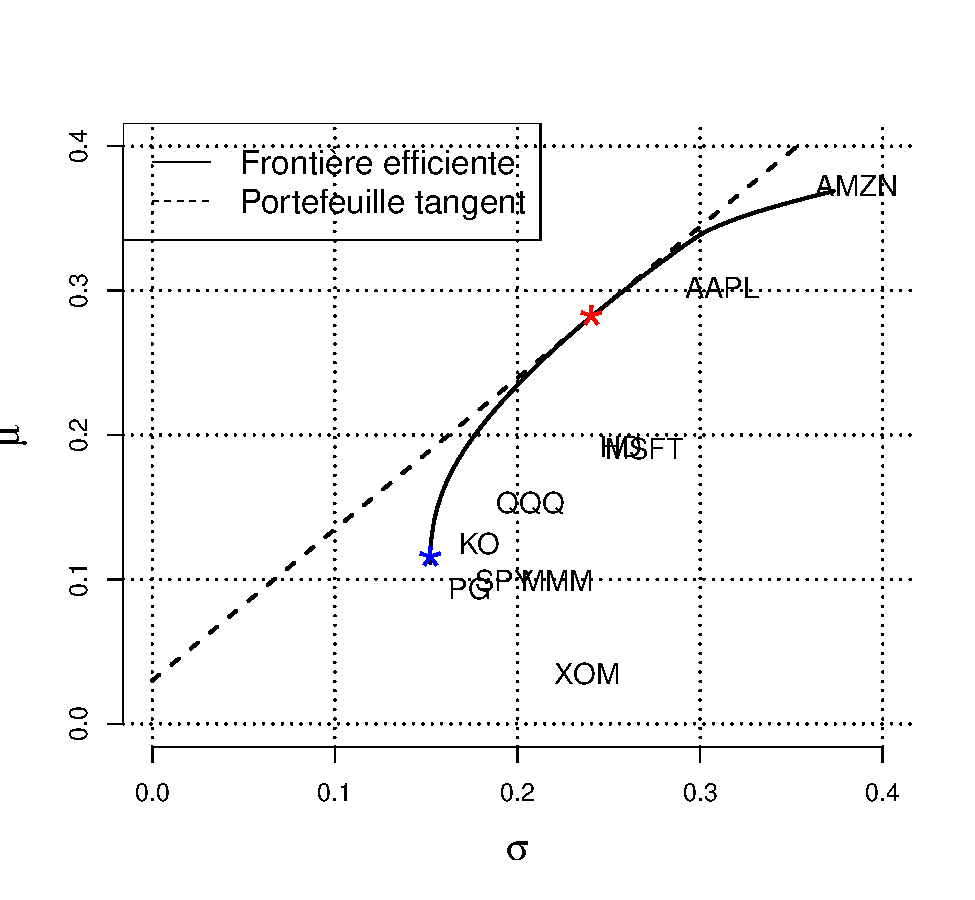
\includegraphics{TP-2_files/figure-latex/unnamed-chunk-11-1.pdf} Sur
ce graphique, le point bleu représente le portefeuille de variance
minimale et le point rouge le portefeuille tangent.

Comme nous l'avons vue précédemment, le portefeuille tangent est peu
varié avec plus de 70\% des allocations réparties sur deux titres
fortement corrélés. Il conviendrait alors d'investir une partie de son
capital dans un actif sans risque pour équilibrer notre portefeuille,
avec un rendement plus faible mais moins risqué.

L'autre solution est de diversifier son portefeuille tangent, en
imposant ajoutant de nouvelles conditions aux allocations des titres.

\begin{itemize}
\tightlist
\item
  Même calcul en ajoutant des contraintes supplémentaires qui vous
  semblent pertinentes (ex: pas plus de 20\% de l'actif risqué alloué à
  un seul titre, etc.)
\end{itemize}

\hypertarget{portefeuille-uxe0-variance-minimale-1}{%
\subsection{Portefeuille à Variance
Minimale}\label{portefeuille-uxe0-variance-minimale-1}}

Avec \(W_i\ge 0\) et \(W_i\le 20%
\) On introduit un nouveau paramètre : \(lim\). Il va nous permettre
d'imposer une valeur maximal au \(w_i\).

\begin{table}

\caption{\label{tab:unnamed-chunk-13}Allocations du portefeuille risqué de varaince minimale avec les poids positifs et inferieurs à 0.2}
\centering
\begin{tabular}[t]{lr}
\toprule
  & Allocations\\
\midrule
AAPL & 0.00000\\
AMZN & 0.00000\\
MSFT & 0.00000\\
F & 0.00000\\
SPY & 0.14010\\
\addlinespace
QQQ & 0.18803\\
XOM & 0.06583\\
MMM & 0.16134\\
HD & 0.04470\\
PG & 0.20000\\
\addlinespace
KO & 0.20000\\
\bottomrule
\end{tabular}
\end{table}

On remarque que les poids sont bien positifs et inferieurs à 20\%. On
peut également noter que le portefeuille de variance minimale est plus
équilibrer.

\hypertarget{calcul-de-la-frontiuxe8re-1}{%
\subsection{Calcul de la Frontière}\label{calcul-de-la-frontiuxe8re-1}}

Avec \(W_i\ge 0\) et \(W_i \le 20%
\)

Puisque nous avons ajouter la contrainte supplémentaire sur les \(w_i\),
la fonction \(solve.QP\) ne trouvait plus de solution pour des rendement
trop élevé. Nous avons donc dû limiter les rendements à 0,24. Nous avons
remarqué que c'est à partir de cette valeur de rendement que la fonction
n'arrivait plus à trouver de solution.

\begin{Shaded}
\begin{Highlighting}[]
\NormalTok{mu.star <-}\StringTok{ }\KeywordTok{seq}\NormalTok{(}\DataTypeTok{from=}\NormalTok{min.ret}\OperatorTok{+}\KeywordTok{abs}\NormalTok{(}\KeywordTok{min}\NormalTok{(mu))}\OperatorTok{/}\DecValTok{100}\NormalTok{, }\DataTypeTok{to=}\FloatTok{0.24}\NormalTok{, }\DataTypeTok{length.out=}\DecValTok{200}\NormalTok{)}
\NormalTok{mu.free <-}\StringTok{ }\FloatTok{0.03}
\NormalTok{sol <-}\StringTok{ }\OtherTok{NULL}
\ControlFlowTok{for}\NormalTok{(mu.s }\ControlFlowTok{in}\NormalTok{ mu.star) \{}
\CommentTok{# constraints: 2 equality}
\NormalTok{A.sum <-}\StringTok{ }\KeywordTok{matrix}\NormalTok{(}\KeywordTok{rep}\NormalTok{(}\DecValTok{1}\NormalTok{,}\KeywordTok{length}\NormalTok{(mu)), }\DataTypeTok{ncol=}\DecValTok{1}\NormalTok{)}
\NormalTok{A.mat <-}\StringTok{ }\KeywordTok{cbind}\NormalTok{(A.sum, mu, }\KeywordTok{diag}\NormalTok{(}\KeywordTok{length}\NormalTok{(mu)),}\OperatorTok{-}\DecValTok{1}\OperatorTok{*}\KeywordTok{diag}\NormalTok{(}\KeywordTok{length}\NormalTok{(mu)))}
\NormalTok{b <-}\StringTok{ }\KeywordTok{c}\NormalTok{(}\DecValTok{1}\NormalTok{, mu.s, }\KeywordTok{rep}\NormalTok{(}\DecValTok{0}\NormalTok{, }\KeywordTok{length}\NormalTok{(mu)),}\KeywordTok{rep}\NormalTok{(}\OperatorTok{-}\NormalTok{lim, }\KeywordTok{length}\NormalTok{(mu)))}
\NormalTok{qp <-}\StringTok{ }\KeywordTok{solve.QP}\NormalTok{(}\DecValTok{2}\OperatorTok{*}\NormalTok{Sigma, }\KeywordTok{rep}\NormalTok{(}\DecValTok{0}\NormalTok{,}\KeywordTok{length}\NormalTok{(mu)), A.mat, b, }\DataTypeTok{meq=}\DecValTok{2}\NormalTok{)}
\NormalTok{sharpe <-}\StringTok{ }\NormalTok{(mu.s }\OperatorTok{-}\StringTok{ }\NormalTok{mu.free) }\OperatorTok{/}\StringTok{ }\KeywordTok{sqrt}\NormalTok{(qp}\OperatorTok{$}\NormalTok{value)}
\NormalTok{  tmp <-}\StringTok{ }\KeywordTok{matrix}\NormalTok{(}\KeywordTok{c}\NormalTok{(mu.s, }\KeywordTok{sqrt}\NormalTok{(qp}\OperatorTok{$}\NormalTok{value), sharpe, qp}\OperatorTok{$}\NormalTok{solution), }\DataTypeTok{nrow=}\DecValTok{1}\NormalTok{)}

\ControlFlowTok{if}\NormalTok{(}\KeywordTok{is.null}\NormalTok{(sol)) \{}
\NormalTok{  sol <-}\StringTok{ }\NormalTok{tmp  }
\NormalTok{\} }\ControlFlowTok{else}\NormalTok{ \{}
\NormalTok{  sol <-}\StringTok{ }\KeywordTok{rbind}\NormalTok{(sol, tmp)}
\NormalTok{\}}
\NormalTok{\}}
\end{Highlighting}
\end{Shaded}

\begin{table}
\caption{\label{tab:unnamed-chunk-16}Portefeuille risqué tangent avec les poids positifs et inferieurs à 0.2}

\centering
\begin{tabular}[t]{lr}
\toprule
  & Allocations\\
\midrule
AAPL & 0.20000\\
AMZN & 0.20000\\
MSFT & 0.09361\\
F & 0.00000\\
SPY & 0.00000\\
\addlinespace
QQQ & 0.00000\\
XOM & 0.00000\\
MMM & 0.00000\\
HD & 0.20000\\
PG & 0.10639\\
\addlinespace
KO & 0.20000\\
\bottomrule
\end{tabular}
\centering
\begin{tabular}[t]{lr}
\toprule
  & Allocations\\
\midrule
mu & 0.22601\\
stdev & 0.19773\\
\bottomrule
\end{tabular}
\end{table}

\hypertarget{ajout-dun-actif-sans-risque-1}{%
\subsection{Ajout d'un actif sans
risque}\label{ajout-dun-actif-sans-risque-1}}

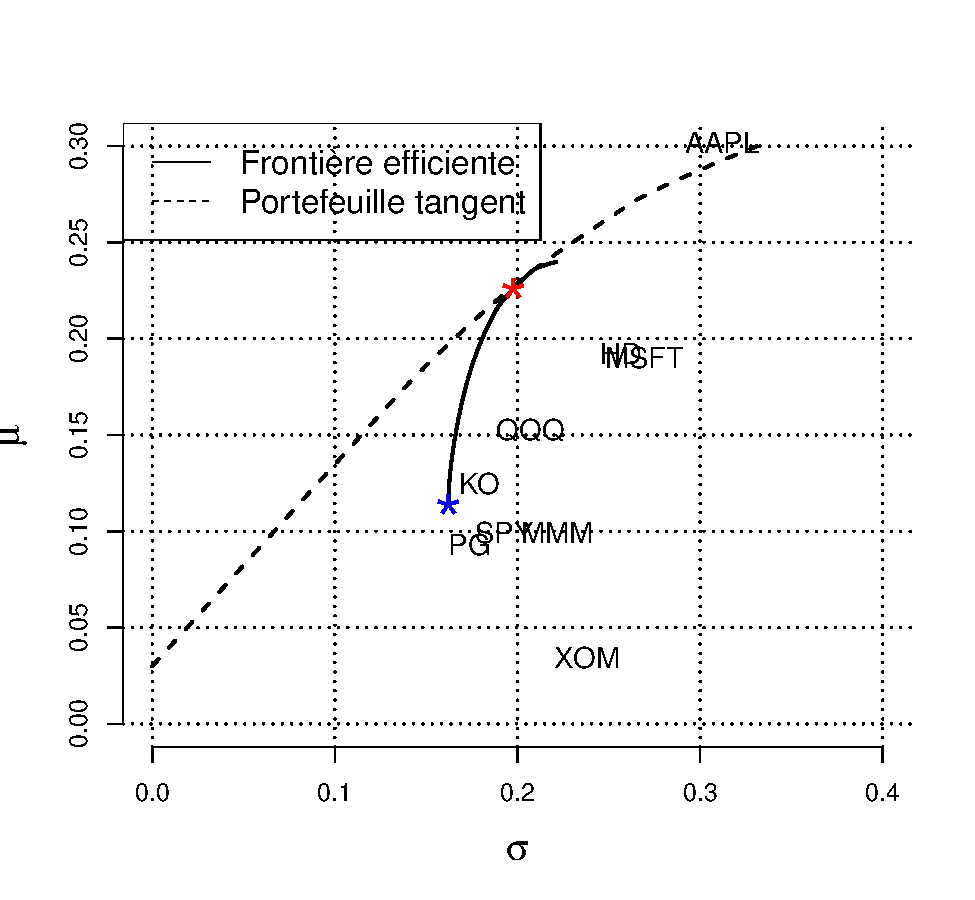
\includegraphics{TP-2_files/figure-latex/unnamed-chunk-17-1.pdf}

Sur ce graphique, le point bleu représente le portefeuille de variance
minimale et le point rouge le portefeuille tangent.

Le portefeuille tangent est plus diversifié avec 4 actions à 20\%
d'allocation chacune : AAPL, AMZN, HD, et KO. Nous pouvons calculer le
rapport \(\frac{\mu}{\sigma}\) pour déterminer si ce portefeuille
tangent est mieux optimisé. Das le cadre de la première partie on
obtient \[\frac{0.28211}{0.24069}=1.1721\] Et dans celui de la seconde :
\[\frac{0.22601}{0.19773}=1.1430\] On remarque donc que ce rapport est
plus avantageux sans limiter les \(w_i\) à 20\%. À la question 1, le
portefeuille tangent était composé à plus de 70\% d'AAPL et de AMZN. On
peut donc en déduire que les actions AAPL et AMZN ont un fort rendement
ce qui est confirmé par le tableau 1. Cependant, le tableau 2 nous
montre que KO est l'une des actions les moins corrélés avec AAPL et
AMZN. D'autre part, notre portefeuille contient également 10\% de PG,
qui est l'action la moins corrélé avec AMZN et AAPL. Tout cela nous a
permis de diversifier notre portefeuille et donc de diminuer le risque.
Il faut cependant nuancer notre analyse car bien que ces actions soient
les moins corrélés de l'indice, leurs corrélations restent relativement
élevées (aux alentours de 30\%).

\end{document}
